\documentclass[a4paper,11pt]{article}
% Use ctrl + alt + V to view live pdf

% Packages
\usepackage[utf8]{inputenc} % For encoding
\usepackage[T1]{fontenc} % Better handling of accented characters and hyphenation
\usepackage{microtype} % Improves spacing and justification
\usepackage{amsmath, amssymb} % For equations and symbols
\usepackage{graphicx} % For including graphics/images
\usepackage{caption} % For customizing figure and table captions
\usepackage{subcaption} % For subfigures and subcaptions
\usepackage{float} % For fixing figure and table positions
\usepackage{booktabs} % For professional-looking tables
\usepackage{siunitx} % For consistent typesetting of units and numbers
\usepackage[margin=2cm]{geometry} % Adjusts page margins
\usepackage{fancyhdr} % For custom headers and footers
\usepackage{lmodern} % For a professional-looking font (main body font)
\usepackage{titlesec} % For title customization
\usepackage{array} % For custom table formatting
\usepackage[colorlinks=true, linkcolor=black, citecolor=blue, urlcolor=blue]{hyperref} % Colored links without boxes
\usepackage{cleveref} % For improved cross-referencing    
\usepackage{multirow}
\usepackage{enumitem}
\usepackage{listings}
\usepackage{xcolor}
\usepackage{textcomp}
\usepackage{tabularx}
\usepackage{changepage}
\usepackage{tikz}
\usepackage{pdfpages}
\usepackage[table]{xcolor}
\usetikzlibrary{shapes.geometric, arrows}
% --- C++ Style ---
\lstdefinestyle{cpp-style}{
    language=C++,
    basicstyle=\ttfamily\footnotesize,
    keywordstyle=\color{blue}\bfseries,
    stringstyle=\color{orange},
    commentstyle=\color{gray}\itshape,
    numbers=left,
    numberstyle=\tiny\color{gray},
    numbersep=10pt,
    backgroundcolor=\color{white},
    showspaces=false,
    showstringspaces=false,
    breaklines=true,
    breakatwhitespace=true,
    tabsize=4,
    captionpos=b,
    frame=single,
    rulecolor=\color{black},
}

% --- Python Style ---
\lstdefinestyle{python-style}{
    language=Python,
    basicstyle=\ttfamily\footnotesize,
    keywordstyle=\color{blue}\bfseries,
    commentstyle=\color{gray}\itshape,
    stringstyle=\color{green!50!black},
    frame=single,
    breaklines=true,
    showstringspaces=false,
    captionpos=b
}
\renewcommand{\lstlistingname}{Code}
% Custom settings
\pagestyle{fancy}
\fancyhf{}
\fancyhead[L]{\textit{SF4 - DataLogger}} % Header left
\fancyhead[R]{\textit{Will Hewes - wh365}} % Header right 
\fancyfoot[C]{\thepage} % Footer center
\setlength{\headheight}{15pt} % Header height
\setlength{\parindent}{0em} % Indentation for paragraphs
\setlength{\parskip}{0.5em} % Add spacing between paragraphs
\setlength{\abovedisplayskip}{1em}
\setlength{\belowdisplayskip}{1em}
\setlength{\abovedisplayshortskip}{1em}
\setlength{\belowdisplayshortskip}{1em}
% \setlist{topsep=0.2em, partopsep=0em, itemsep=0.1em, parsep=0em}

\graphicspath{{Images/}}

% \renewcommand{\arraystretch}{1.2}

% Title formatting
\renewcommand{\maketitle}{
    \begin{center}
        \LARGE \textbf{ENGINEERING TRIPOS PART IIA} \\[0.5em]
        \Large \textbf{SF4 - DataLogger} \\[0.5em]
        \textbf{Final Report} \\[1.5em]
        \vspace{-1em}
        \small Will Hewes - wh365 \\ 
        Pembroke College \\ 
        \vspace{0.5em}
    \end{center}
}

\begin{document}
\pagenumbering{gobble}
% 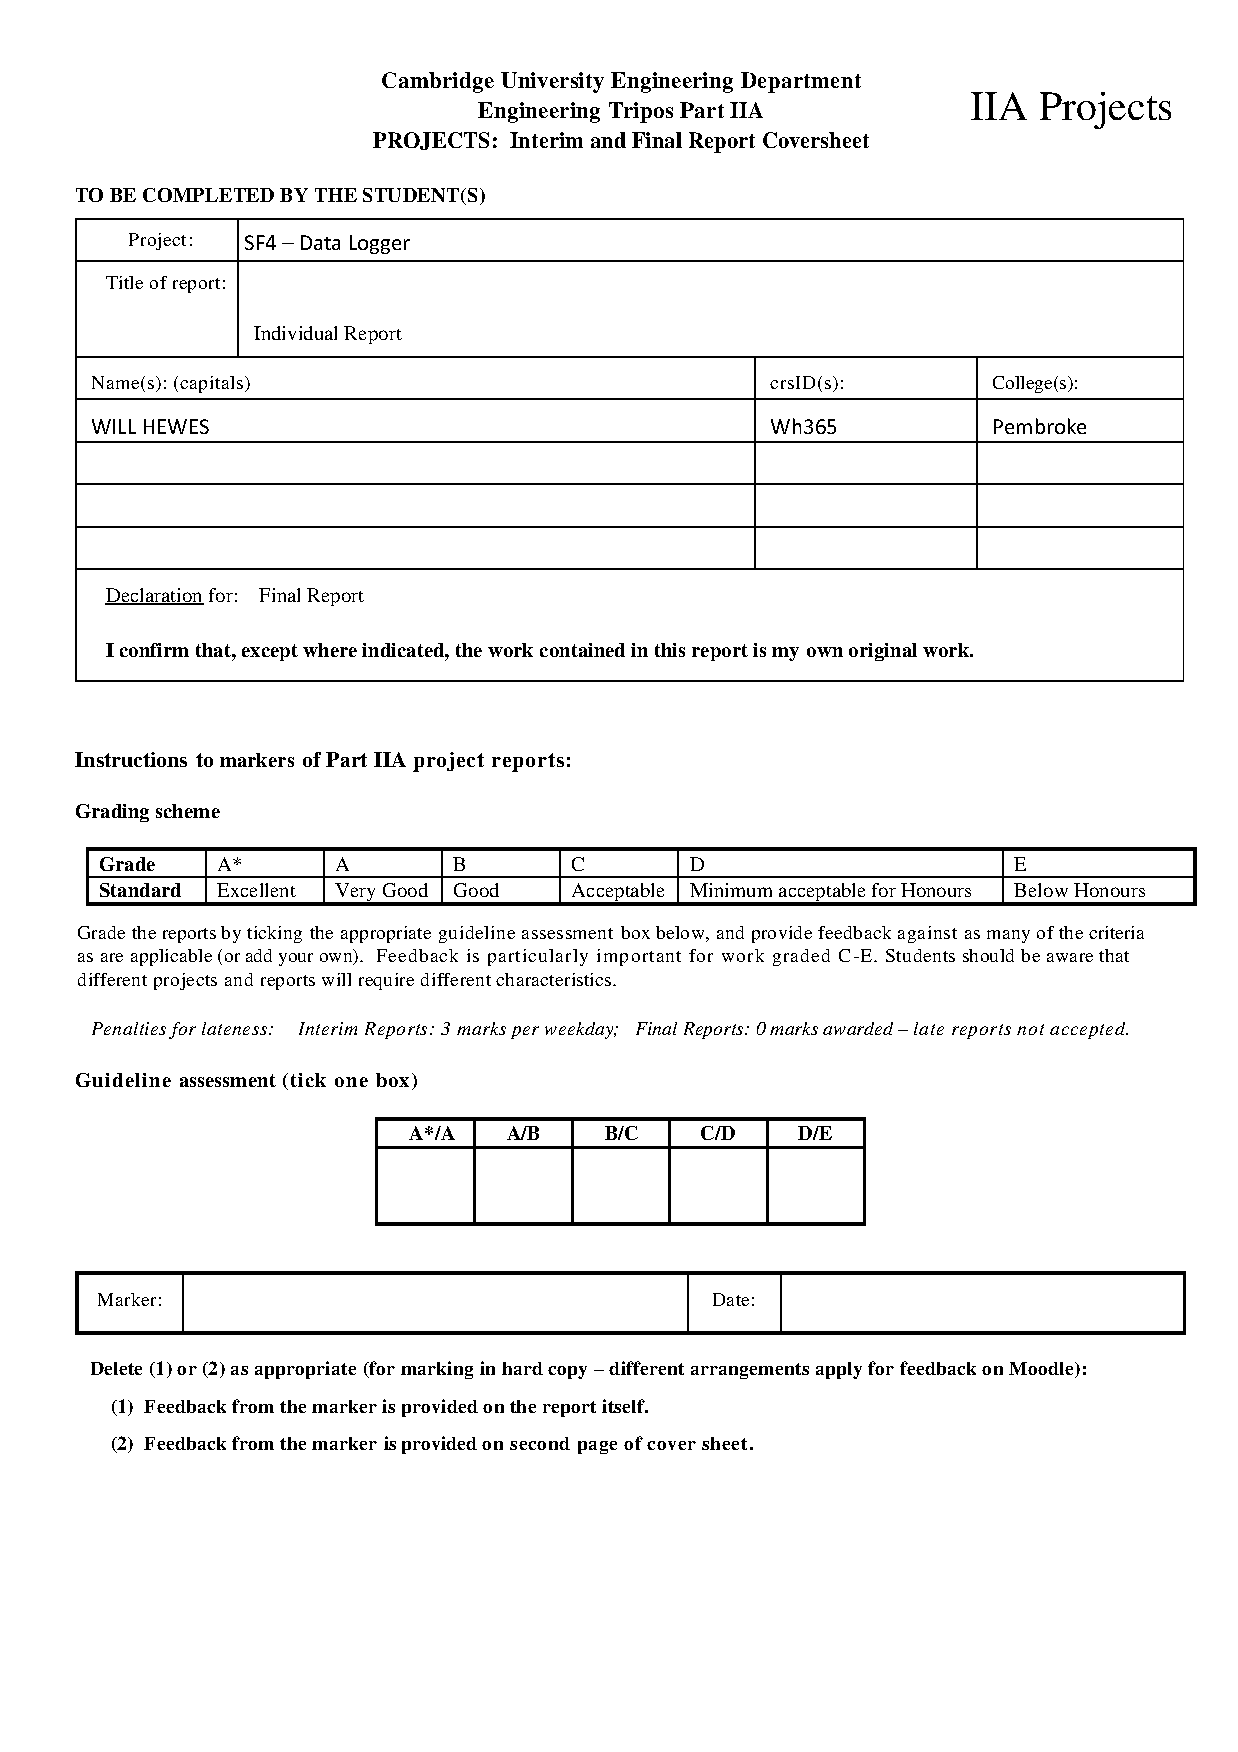
\includepdf[pages=-]{Handouts/IIA_Project_Coversheet Final Report.pdf}
\maketitle
\hrule
\tableofcontents
\newpage
\pagenumbering{arabic} \setcounter{page}{1}

\section{Introduction}
\label{sec:introduction}

The aim of this project was to develop a microcontroller-based 
automatic plant watering system.
The system can autonomously monitor soil moisture levels, 
plot the data over time, and provide options to water the plant
manually when required or in response to threshold moisture levels.
This allows for effective monitoring and care with minimal user intervention.

In addition to moisture sensing, the system also tracks temperature, 
and was supposed to track humidity and light -
though this could not be implemented due to component delivery delays.
This means most of the key factors affecting plant health
can be closely tracked, enabling detailed analysis of
optimum conditions for plant health.
These additional features enhance the system's utility for targeted care for the plants,
or for more sophisticated control and research.

The motivation behind creating this autonomous watering system was twofold. 
Firstly, it can be used as demonstrated on a small scale,
allowing direct control over the conditions of one 
or a small number of houseplants,
offering a convenient way to care for plants.
This will remove the majority of the care required
to look after these often frail plants,
which is particularly useful over holidays or 
during the hot Summer months.
As a university student with several well-loved plants,
this has immediate personal appeal.

On a larger scale, the system provides a modular, 
low-cost framework adaptable to industrial or agricultural applications, 
where automated irrigation and environmental monitoring are increasingly valuable.
The low cost and simple design of the system will be appealing 
to widespread, versatile integration,
and the ease with which components can be added
and the GUI can be customised will allow for rapid expansion into various sectors.

\section{System Summary}
\label{sec:summary}

The final system comprises a microcontroller
connected via USB serial to a Python-based PC interface. 
The microcontroller collects real-time data from a capacitive soil moisture sensor 
and a TMP36 temperature sensor, formats the data, 
and transmits it at regular, rapid intervals. 
The PC software receives the data, displays it graphically, 
and writes it to a timestamped CSV log.

The watering mechanism is controlled by a mini servo motor 
which actuates a 3D-printed pinch valve connected to a reservoir. 
Watering can be triggered manually from the graphical user interface, 
or automatically when the measured soil moisture drops below 
a configurable threshold. 
This enables a complete closed-loop feedback system 
between environmental sensing, control logic, 
and physical actuation.

The GUI also provides users with real-time feedback, 
warning indicators for out-of-range values, 
and basic controls for adjusting system thresholds and modes. 
Operation is intended to be simple, low-maintenance, 
and suitable for unattended deployment over extended periods.

While targeted toward small-scale domestic use, 
the system's modular design allows for straightforward expansion. 
Additional sensors (e.g., humidity, light), 
alternative actuators, or wireless communication modules 
can be added with minimal reconfiguration, 
making the platform a flexible basis for 
larger agricultural or environmental monitoring systems.

\section{Project Management}
\label{sec:project_management}

The project was developed collaboratively in a two-person team, 
with both members working on the system holistically,
applying changes to each module incrementally
as the product was slowly developed.
This approach was taken as opposed to a divided approach,
wherein each member would manage either software or firmware,
with the intention of giving each of us a better understanding 
and overview of the system as a whole,
allowing us to effectively contribute ideas 
concerning the whole project collaboratively. 
This had the consequence that on occasion we would 
both be making changes to the same module simultaneously.

By nature of this development style,
there was an increased risk of conflicts introduced to the system
if we did not take proper care to ensure that our changes were compatable.
As a result, version control and clear communication 
became a vital aspect of our project management.

Version control and collaborative development were managed using GitHub, 
enabling parallel work on the codebase
and simplifying the process of merging changes and tracking development history. 
This also allowed modular elements - 
such as the GUI framework and firmware routines -
to be developed and tested in isolation before being brought together.

The project followed a phased development structure:
\begin{enumerate}[nosep]
    \item \textbf{Component Validation:} 
    Initial sessions focused on ordering the individual sensors 
    and actuators then evaluating them through breadboard testing, 
    ensuring reliable signal acquisition and control.
    \item \textbf{Prototype Development:} 
    In parallel with circuit construction, a socket-based simulation 
    of the Arduino-PC interface was created to support 
    early development of the GUI and data parsing routines 
    in the absence of hardware.
    \item \textbf{System Integration and Testing:} 
    Once physical components were functional, development transitioned 
    to serial communication over USB. 
    Modules were progressively integrated and tested together 
    in a final working system.
\end{enumerate}

Throughout the project, care was taken to adopt a modular workflow, 
with each subcomponent independently tested and versioned. 
This reduced the risk of cascading failures during integration and 
supported incremental development even in the face of hardware delays 
or debugging setbacks.

\section{System Architecture}
\label{sec:architecture}

\subsection{Block Diagram}
\label{sec:block_diagram}

Figure \ref{fig:Block_Diagram_for_the_automatic_watering_system} below presents a high-level overview 
of the system architecture, outlining the key components and their interactions. 
At the centre is the Arduino Uno microcontroller, responsible for interfacing with 
the sensors and controlling the servo-driven watering mechanism. 
It collects analogue data from the soil moisture and temperature sensors, 
processes it internally, and transmits formatted readings 
to the host PC via a serial USB connection.

The PC software receives this data stream and handles real-time visualisation
and CSV logging.
The user can configure system parameters through a graphical user interface, 
which sends commands back to the Arduino to adjust moisture thresholds, 
trigger watering, or enable warning indicators.

The servo receives control signals from the Arduino and actuates a 3D-printed pinch valve 
attached to a water reservoir, allowing precise water delivery to the plant. 
While only moisture and temperature sensors were fully integrated, 
additional sensor channels were reserved on the PCB layout for light and humidity, 
ensuring system extensibility for future work.

\begin{figure}[H]
    \centering
    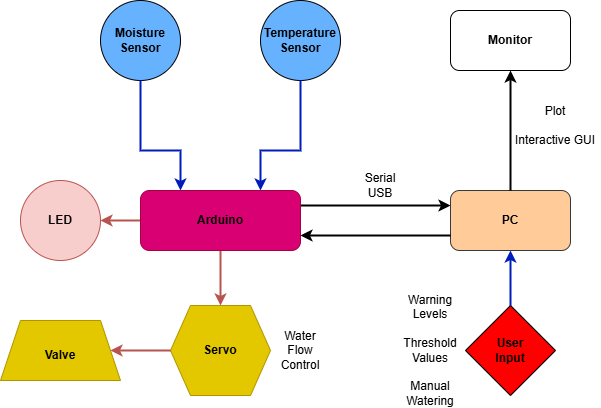
\includegraphics[width=0.8\textwidth]{Datalogger Block Diagram - final.png}
    \caption{Block Diagram for the automatic watering system}
    \label{fig:Block_Diagram_for_the_automatic_watering_system}
\end{figure}

\subsection{Component Orders}
\label{sec:Components}
The physical system was built around a small set of carefully chosen components, 
ordered through Farnell. 
The sensors included a capacitive soil moisture sensor, 
chosen due to its improved output stability and longevity compared to a resistive module,
and a TMP36 temperature sensor for simple analogue interfacing, 
which required a 100pF capacitor acting in parallel between its output pin and the ground
in order to stabilise its readings, 
as well as the incorporation of an AREF wire.

A mini servo motor was selected to control the water delivery mechanism, 
providing reliable actuation of a 3D-printed pinch valve.
This likewise had a capacitor placed between its power and ground pins 
to limit current spikes and provide a smoother, controlled motion.

Additional sensors for humidity and light intensity were also ordered, 
but were not included in the final system due to shipping delays. 
Nonetheless, space was reserved within the system design 
for their future integration.

These components are shown in Table \ref{tab:component_order} below,
with the unused sensors highlighted in yellow.
With a budget of £15, there was a remaining £3.65 
that could be used for integration of more sensors,
or replacing current sensors with a higher quality alternative.

\begin{table}[H]
    \centering
    \renewcommand{\arraystretch}{1.5} 
    \makebox[\linewidth][c]{
    \resizebox{0.8\textwidth}{!}{
    \begin{tabular}{|c|c|c|}
        \hline
        \textbf{Order Code} & \textbf{Description of Component} & \textbf{Unit Price (£)} \\
        \hline
        2946124 & Capacitive Soil Moisture Sensor Module & 4.69 \\
        \hline
        SC21096 & Mini servo & 2.94 \\
        \hline
        4030054 & Temperature sensor & 1.38 \\
        \hline
        \rowcolor{yellow!60} 3167525 & Light sensor & 1.43 \\
        \hline
        \rowcolor{yellow!60} SN36746 & Humidity sensor & 0.91 \\
        \hline
        \multicolumn{2}{|c|}{\textbf{\large Total}} & \textbf{\large 11.35} \\
        \hline
    \end{tabular}
    }   
    }
    \caption{Component Order Summary}
    \label{tab:component_order}
\end{table}

\subsection{Circuit Design}
\label{sec:circuit_design}

The final circuit design consisted of a single Arduino Uno board interfacing 
with two analogue sensors and a mini servo motor. The sensors were connected 
to analogue input pins, with the soil moisture sensor wired directly and the 
TMP36 temperature sensor routed through a \SI{100}{\pico\farad} capacitor 
between its signal and ground pins to suppress high-frequency noise,
improving stability of the output signal. 
The Arduino's \texttt{AREF} pin was set to an external \SI{3.3}{\volt} reference 
to improve ADC resolution and match the expected sensor output range.
The servo motor required a \SI{100}{\micro\farad} decoupling capacitor added between 
its power and ground pins to limit voltage dips during actuation.

The complete analogue circuit layout is shown in 
Figure~\ref{fig:Analogue_Circuit_Diagram_for_the_automatic_watering_system}.

\begin{figure}[H]
    \centering
    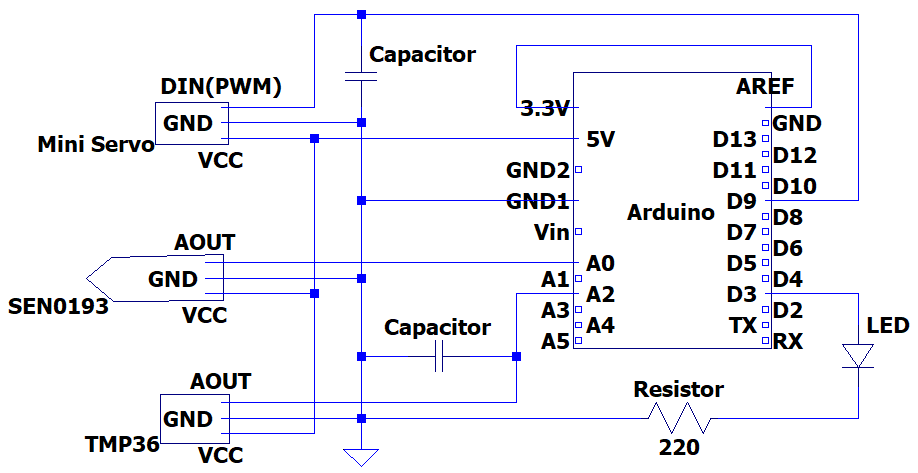
\includegraphics[width=0.8\textwidth]{Analogue Circuit Diagram - final.png}
    \caption{Analogue Circuit Diagram for the automatic watering system}
    \label{fig:Analogue_Circuit_Diagram_for_the_automatic_watering_system}
\end{figure}

\subsection{Watering Mechanism}
\label{sec:water_system}

The water delivery system was implemented using the mini servo motor to actuate a 
3D-printed pinch valve \cite{pinch_valve_design}. 
This design was selected due to its ease of implementation, compact size, 
and small number of parts,
reducing the risk of any mechanical faults within the system. 
The open-source valve design was scaled up 
to fit the PVC tubing we had on hand to connect.

The servo applies a clamping force to compress the tubing, restricting flow when closed 
and releasing it when opened. This mechanism provided a reliable and cost-effective 
alternative to traditional solenoid valves or pump systems, which tend to require 
greater current draw and more complex power handling.

A moisture threshold, configured via the PC interface, controlled automatic actuation. 
When the measured moisture dropped below this value stored on the Arduino, 
the servo was triggered to open the valve for a set duration, 
delivering a fixed amount of water. 
Manual triggering was also available through the GUI.
\iffalse
Although the current implementation assumes a fixed water level in the reservoir, 
the design allows for future integration of a float switch or liquid level sensor 
to prevent dry actuation and ensure continued reliability in unattended use. 
\fi
The actuation logic, timing, and safety handling are further detailed in 
Section~\ref{subsec:main_loop}.

\section{Initial Development}
\label{sec:initial_development}
\subsection{Sensor Prototyping}
\label{sec:sensor_prototyping}
\subsection{GUI}
\label{sec:gui_simulation}
\subsection{Communication Protocol}
\label{sec:comm_protocol}

\section{Final Implementation}
\label{sec:final_implementation}
\subsection{Firmware}
\label{sec:firmware}
\subsubsection{Main Loop}
\label{subsec:main_loop}
\subsubsection{Signal Processing}
\label{subsec:firmware_processing}
\subsection{Software}
\label{sec:software}
\subsubsection{Module Structure}
\label{subsec:software_modules}
\subsubsection{User Interface}
\label{subsec:software_ui}

\section{Technical Challenges}
\label{sec:technical_problems}

\section{Further Improvements}
\label{sec:further_improvements}

\section{Conclusion}
\label{sec:conclusion}


\newpage
\appendix
\begin{thebibliography}{9}

\bibitem{arduino_servo}
Arduino. \textit{Servo Motor Basics with Arduino} : \\
\url{https://docs.arduino.cc/learn/electronics/servo-motors/}

\bibitem{tmp36}
Analog Devices. \textit{TMP35/TMP36/TMP37 Data Sheet} : \\
\url{https://www.analog.com/en/products/tmp36.html} 

\bibitem{arduino_tmp36}
ArduinoGetStarted. \textit{Arduino - TMP36 Temperature Sensor} : \\
\url{https://arduinogetstarted.com/tutorials/arduino-tmp36-temperature-sensor}

\bibitem{dfrobot}
DFRobot. \textit{Capacitive Soil Moisture Sensor SKU SEN0193} : \\
\url{https://wiki.dfrobot.com/Capacitive_Soil_Moisture_Sensor_SKU_SEN0193}

\bibitem{pinch_valve_design}
Printables. \textit{Pinch Valve Powered by Servo} : \\
\url{https://www.printables.com/model/247744-pinch-valve-powered-by-servo/files}

\end{thebibliography}

\section{Interim Report}
% 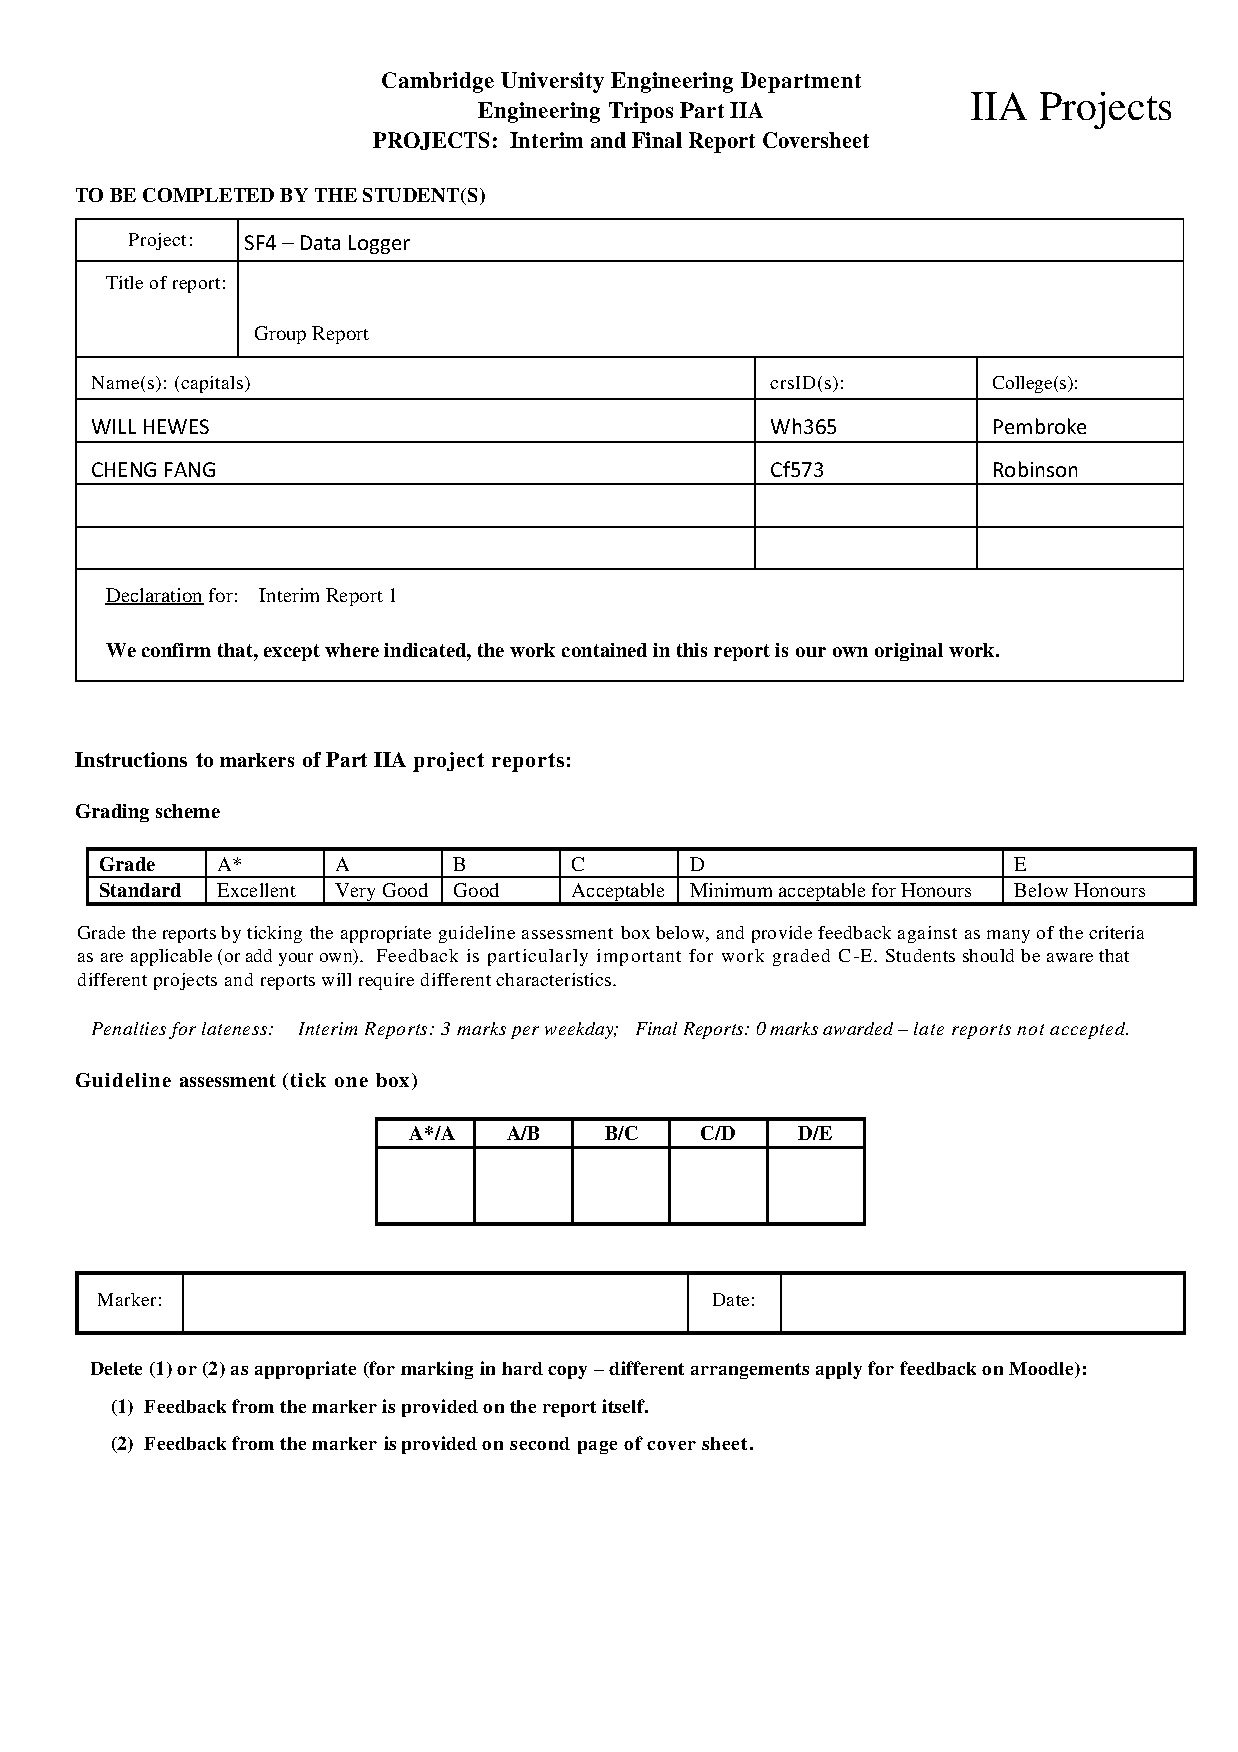
\includepdf[pages=-]{Reports/First Interim Report.pdf} % e.g. [pages={1,3-5,7}] to include pages 1,3,4,5,7
% Featuring the Interim Report

\end{document}